%
% General structure for the revdetua class:
%
\documentclass[portugues,final]{revdetua}
\usepackage[portuguese]{babel}
\usepackage{listingsutf8}
\usepackage[utf8]{inputenc}
\usepackage[T1]{fontenc}
\usepackage{graphicx}
\usepackage{hyperref}
\usepackage{wrapfig}
\usepackage{float}
\usepackage{color}
\usepackage{eurosym}
%
% Valid options are:
%
%   longpaper --------- \part and \tableofcontents defined
%   shortpaper -------- \part and \tableofcontents not defined (default)
%
%   english ----------- main language is English (default)
%   portugues --------- main language is Portuguese
%
%   draft ------------- draft version
%   final ------------- final version (default)
%
%   times ------------- use times (postscript) fonts for text
%
%   mirror ------------ prints a mirror image of the paper (with dvips)
%
%   visiblelabels ----- \SL, \SN, \SP, \EL, \EN, etc. defined
%   invisiblelabels --- \SL, \SN, \SP, \EL, \EN, etc. not defined (default)
%
% Note: the final version should use the times fonts
% Note: the really final version should also use the mirror option
%

\begin{document}

% Note: the month must be in Portuguese

\title{\textbf{Álbum de fotos 3D implementado com OpenCV e OpenGL} \\ Computação Visual\\Universidade de Aveiro}
\author{Diogo Silva 60337}
\maketitle
\begin{resumo} % Note: in Portuguese
Este relatório descreve detalhadamente a estrutura, filtros e o motor da aplicação implementada em OpenGL e OpenCV.
Descrevendo detalhadamente, método de manipulação, método de visualização, entre outros.
\end{resumo}

\section*{Nota}
Toda a documentação relativa a complicação encontra-se num ficheiro à parte com o nome README (aconselha-se que seja lido antes de tentar executar a aplicação desenvolvida), ou no fim deste relatório.
\section{Estrutura da Aplicação}

A aplicação está organizada de forma a ser reutilizável, sendo assim, existe várias componentes distintas:
\begin{enumerate}
\item Efeitos, manipulação de cada imagem, mais precisamente, aplicação de filtros sobre imagens, tendo um modo personalizado ou com valores de entrada por defeito
\item Modelos, contém todas as caracterísiticas necessárias para a representação de um modelo no ambiente OpenGL
\item Shaders, trata do fazer o processamento respectivo na placa gráfica
\item Utilidades, contém as utilidades para o sistema, neste momento, contém apenas MathUtils que permite manipular matrizes e vectores
\item Visualizador Gráfico (animações), manipulação de vários modelos para criar animações, contendo as respectivas acções, como primir um botão
\end{enumerate}

Podendo assim facilmente adicionar um tema gráfico com novas animações, ou adicionar novos filtros ao sistema.

\subsection{Implementação}

Neste capítulo é abordado todas as implementações das classes principais, deixando de lado, classes que herdem interfaces, sendo essas interfaces abordadas.

\subsubsection{Efeitos}

Nesta secção é abordado a implementação da estrutura efeitos e não o detalhe de cada filtro, esse assunto é abordado na secção de Aspectos Importantes do Trabalho.\\

A class {\tt Effect} no ficheiro {\tt effects/effect.{h|c}pp} contém a interface usada por qualquer efeito, sendo que cada filtro vai ter de herdar esta classe de forma a ficar um sistema escalável, sendo que a função principal desta classe é a {\tt ApplyEffect} que faz a respectiva manipulação de cada imagem consoante o filtro de que se trata.\\

Na seguinte imagem é possível verificar a implementação da respectiva classe:

\begin{figure}[h]
\centerline{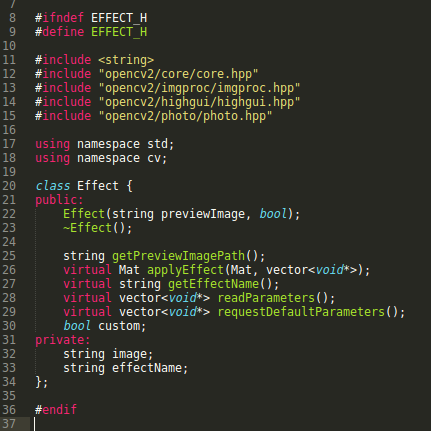
\includegraphics[width=230pt]{images/effect.png}}
\caption{Implementação do Effect}
\label{img:complete}
\end{figure}

Para além desta classe, ainda existe outra classe que permite armazenar todos os filtros existentes fazendo a manipulação deles a partir dela, tendo a mesma a função {\tt ApplyEffect} mas com um campo adicional que indica o filtro respectivo.\\

Esta classe armazena todos os filtros existentes na sua construção (ou seja, no construtor), armazenando-os todos num vector de Effect fazendo assim proveito do polimorfismo.\\

\break
Como se pode ver na imagem seguinte esta classe é muito parecido à {\tt Effect} com a excepção que tem um vector de Effect.

%\begin{figure}[H]
%\centerline{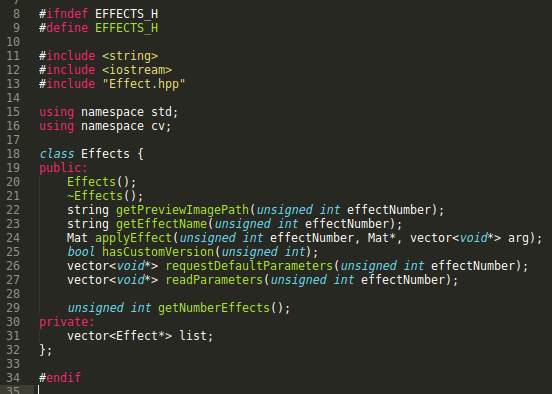
\includegraphics[width=230pt]{images/effects.png}}
%\caption{Implementação do Effects}
%\label{img:complete}
%\end{figure}

\subsubsection{Modelos}

Todos os modelos que precisam de ser representados em OpenGL são carregados para uma classe chamada {\tt GraphicModel} que permite guardar a seguinte informação:
\begin{enumerate}
\item{Número de vertíces}
\item{Lista de vertíces}
\item{Lista das normais}
\item{Lista das texturas}
\item{Matrix da imagem representada}
\item{Matrix da imagem carregada inicialmente}
\item{Valores de deslocamento, rotação e de redimensionamento}
\item{ID da textura actual}
\end{enumerate}

Como se pode verificar na imagem seguinte:

\begin{figure}[H]
\centerline{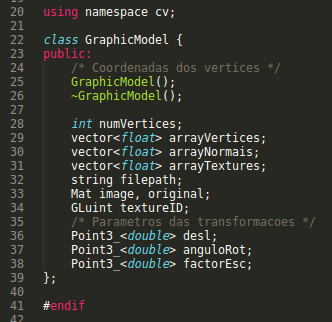
\includegraphics[width=230pt]{images/graphicmodel.png}}
\caption{Implementação do GraphicModel}
\label{img:complete}
\end{figure}

Em que estes dados todos são úteis para a representação no modelo no ambiente gráfico, a excepção da Matrix inicial carregada que serve para dar a possibilidade ao utilizador de voltar a imagem inicial.

\subsubsection{Controlador de temas}

Tal como nos efeitos, para os temas da representação gráfica existe uma classe que funciona como uma interface que permite criar outros temas herdando essa classe, que é a {\tt Theme} no ficheiro {\tt visualization/theme.{h|c}pp}.\\

Essa classe tem todas as funções respectivas aos movimentos básicos, tais como, mover o tema para a direita, para a esquerda, para baixo, ampliar, entre os restantes. Para a implementação de cada tema é passado os modelos gráficos de todas as imagens carregadas do directório, sendo esta classe responsável pela manipulação das suas respectivas deslocações e orientações.\\

Como se pode ver na imagem seguinte, temos a interface pronta a ser herdada por qualquer tema que se pretenda que seja criado.

\begin{figure}[H]
\centerline{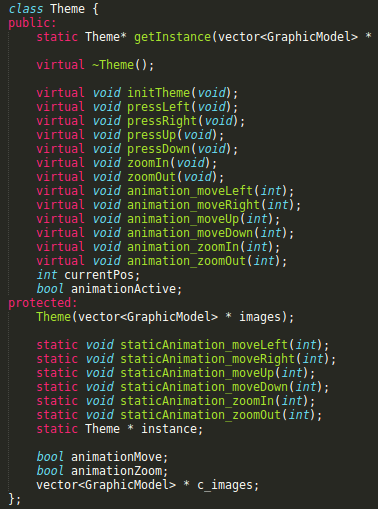
\includegraphics[width=230pt]{images/theme.png}}
\caption{Implementação do Effect}
\label{img:complete}
\end{figure}

Sendo que tanto o tema Coverflow, ou Slideflow herdam esta classe.\\

Para além desta classe, ainda temos um controlador de temas que permite manusear todos os temas introduzidos no sistemas, tendo como um vector de {\tt Theme}, tal como acontecia com a classe {\tt Effects}.\\

Criando assim abstração ao utilizador da manipulação do vector, precisando apenas de fazer {\tt next()} no objecto {\tt ThemeController}.\\

Todos os tipos de visualização criados são abordados no capítulo de ``Aspectos Importantes do Trabalho'' de forma detalhada incluindo uma amostra das suas funcionalidades.\break

\section{Aspectos Importantes do Trabalho}

\subsection{Filtros/Efeitos}
Foram criados vários filtros para que se permitisse modificar qualquer imagem em tempo real com apenas um clique, sendo assim criado vários filtros, tais como: Sepia, Lomo, Tons de Cinza, Pencil Sketch, entre outros.

Considere-se para todos os filtros a seguir referidos, a seguinte imagem original:
\begin{figure}[H]
\centerline{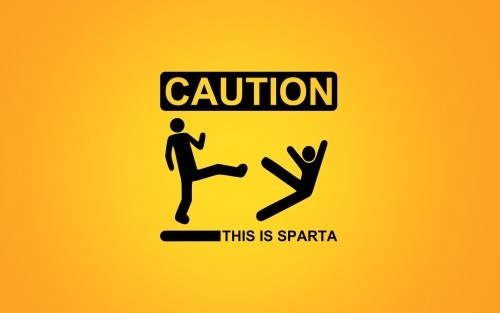
\includegraphics[width=230pt]{images/original.jpeg}}
\caption{Original}
\label{img:complete}
\end{figure}

\subsubsection{Sepia}
Este filtro consiste em aplicar em cada canal de um pixel um factor que é resultado do conjunto dos 3 canais, partindo disto, pode-se já concluir que não é aplicável a imagens com apenas 1 canal.\\

Sendo que os factores\cite{sepia} aplicados a cada canal são os seguintes:\\

$Novo R = 0.189 R + 0.769 G + 0.393 B$

$Novo G = 0.168 R + 0.686 G + 0.349 B$

$Novo B = 0.131 R + 0.534 G + 0.272 B$

Sendo que o resultado final depois de aplicar o filtro de Sepia é o seguinte:

\begin{figure}[H]
\centerline{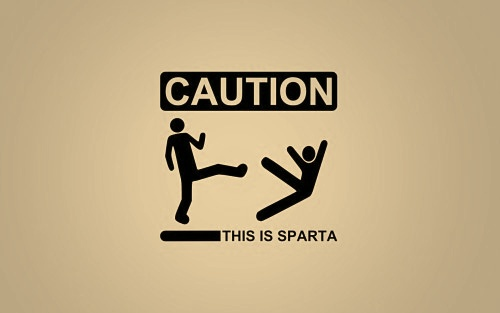
\includegraphics[width=230pt]{images/sepia.jpeg}}
\caption{Sepia}
\label{img:complete}
\end{figure}

Para realizar este efeito em OpenCV, é preciso ler todos os pixeis e em cada pixel substituir cada canal pelo resultado de cada equação, isto pode ser feito de forma mais simples utilizando a função transform de OpenCV que permite aplicar um kernel a matrix de uma imagem.\\

A implementação pode ser encontrada em {\tt effects/types/Sepia.hpp}

\subsubsection{Lomo}
O efeito de Lomo consiste no mesmo que o Sepia mas com a diferença que o resultado do canal vermelho vai para o azul e o resultado do canal azul vai para o canal vermelho, assumindo-se então as seguintes equações.\\

$Novo R = 0.131 R + 0.534 G + 0.272 B$

$Novo G = 0.168 R + 0.686 G + 0.349 B$

$Novo B = 0.189 R + 0.769 G + 0.393 B$

Sendo que o resultado do Sepia e do Lomo são bastante parecidos.

\subsubsection{Tons de cinza}

Este filtro consiste em converter uma imagem em que cada pixel corresponde a um conjunto de 3 canais, para apenas um canal.\\

Sendo que em OpenCV isso se faz de uma forma bastante simples.

{\tt cvtColor(in, image\_out, CV\_BGR2GRAY);}

\subsubsection{Troca de Canais}

A troca de canais consiste em percorrer todos os pixeis 1 a 1 e trocar um canal por outro, por exemplo, o vermelho pelo azul e o azul pelo vermelho.\\

Na aplicação foi implementado este efeito mas em que a troca efectuada seria o canal vermelho pelo verde e vice-versa, sendo que se uma imagem for completamenta vermelha, depois de aplicado este efeito, vai passar a ser toda verde.

\subsubsection{Iluminação}

Para aumentar ou diminuir a iluminação de uma imagem a partir dos canais de cores vermelho, verde e azul é díficil, sendo então que se converte primeiro a imagem para o formato YCbCr.\\

Depois da imagem estar convertida, altera-se directamente o canal Y (canal respectivo da luminosidade), ou seja, multiplica-se por um determinado factor, um Y superior representa uma imagem mais clara e um Y inferior representa uma imagem mais escura.\\

Voltando depois a converter a imagem em RGB.

\subsubsection{Saturação}

Para aumentar ou diminuir a saturação de uma imagem a partir dos canais de cores vermelho, verde e azul é díficil, sendo então que se converte primeiro a imagem para o formato YCbCr, tal como se fazia para iluminação, mas agora em vez de manipular o canal Y, vai se manipular os canais Cb e Cr que representa as diferenças de azul e as diferenças de vermelho, respectivamente.

\subsubsection{Vignette}

O efeito Vignette consiste em fazer desvanecer as bordas de uma imagem, tornando-as mais escuras.\\

Sendo assim pode-se obter este efeito de um forma muito simples, percorrer todos os pixeis da imagem em que para cada pixel calcula-se a distância ao centro, quanto maior a distância, mais escuro a imagem tem de ser, obtendo assim o efeito de Vignette.\\

Para escurecer a imagem, foi multiplicado pelo inverso da distância cada canal de cores, tendo em conta que todos os canais a 0, corresponde ao preto, quando menor for o valor de cada canal, mais escuro fica a imagem.\\

Tendo em conta isto, foi obtido o seguinte resultado:

\begin{figure}[H]
\centerline{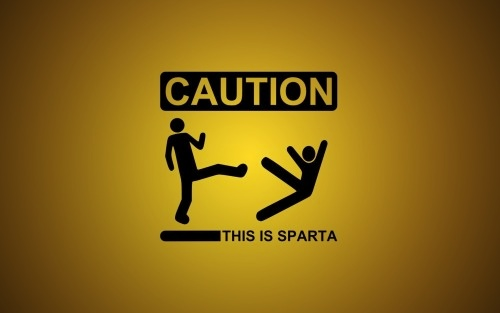
\includegraphics[width=230pt]{images/vignette.jpeg}}
\caption{Vignette}
\label{img:complete}
\end{figure}

\subsubsection{Pencil Sketch}

O efeito pencil sketch tenta imitar o efeito de ter um artista a pintar uma imagem usando um pincel (trabalho manual).\\

Para obter este efeito foi aplicado o seguinte procedimento:
\begin{enumerate}
\item Sobel sobre X
\item Sobel sobre Y
\item Potência de 2 sobre o resultado de cada Sobel e somar
\item Conversão em níveis de cinzento
\item Aplicar o negativo a imagem de forma a tornar o resultado real
\end{enumerate} 

Aplicar o sobel serve para criar os efeitos dos riscos do pincel, fazem a potência e somar serve para juntar apenas os resultados de ambos os Sobels, sendo que depois era preciso converter para os tons habituais que se trabalha normalmente, neste caso, para tons de cinzento, só que ainda não se tem o efeito pretendido pois a imagem encontra-se invertida, sendo assim, aplica-se o negativo da imagem para obter um resultado realístico.\\

Sendo que o resultado final deste processo é o seguinte:

\begin{figure}[H]
\centerline{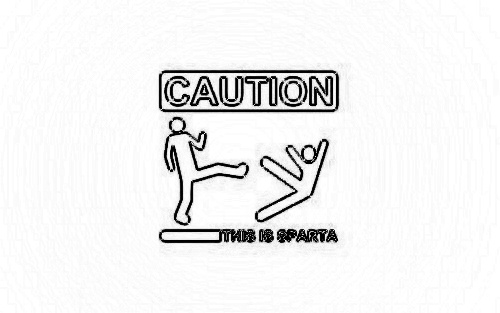
\includegraphics[width=230pt]{images/pencil.jpeg}}
\caption{Pencil Sketch}
\label{img:complete}
\end{figure}

\subsubsection{Cartoon}

Este efeito tem como objectivo obter uma imagem realistica, por exemplo de uma paisagem, e torna-la num cartoon (algo perto de desenho animado).\\

Para obter este efeito foi efecutado em cada pixel uma média dos seus valores a volta sobrepondo o valor actual\cite{seg}, fazendo assim com que pequenas alterações de valores nos canais de cor desapareceçam, fazendo com que a imagem contenha apenas variações de cores mais bruscas, tal como são os desenhos animados.\\

Depois ainda se aplicou Canny para denotar onde essas diferenças apareciam, de forma a dar o contorno ao cartoon.

\subsubsection{Canny}

É apenas aplicação directa da função de OpenCV para detecção de arestas, permitindo o utilizador alterar valores.

\section{Modos de visualização}

Foram criados dois modos de visualização distintos, Coverflow e Slideflow.\\

Ambos os modos de visualização tem a selecção de filtros/efeitos, abertura da câmera, ampliação total da imagem e os botões de interacção com o utilizador implementados da mesma forma, sendo que não é possível alterar sem mexer na estrutura.\\

Tudo o resto é possível alterar criando apenas uma classe que herde a class {\tt Theme}.

Os efeitos de ampliação total e representação da câmera aparecem no capítulo resultado final, tudo o resto apenas é possível executando a aplicação.
\break

\subsection{Coverflow}

Coverflow consiste em gerar as imagens todas numa linha em que o utilizador tem a possibilidade de andar apenas da esquerda para a direita ou da direita para a esquerda.

\begin{figure}[H]
\centerline{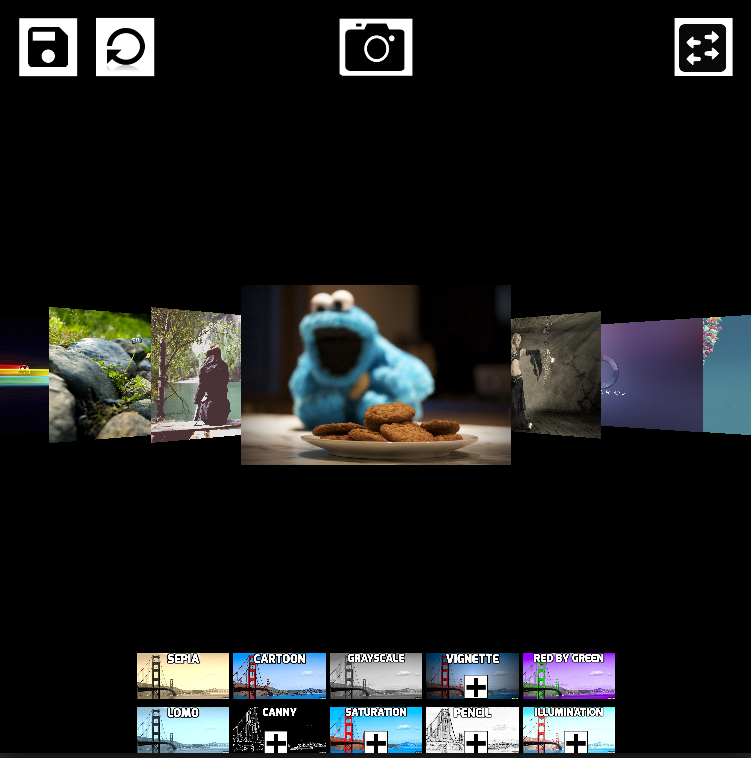
\includegraphics[width=230pt]{images/coverflow.png}}
\caption{Coverflow}
\label{img:complete}
\end{figure}

\subsection{Slideshow}

Slideflow consiste em gerar as imagens todas numa matrix de n columas por m linhas, neste caso, foi implementado com 3 linhas em que o número de colunas é determinado consoante o número de imagens.

\begin{figure}[H]
\centerline{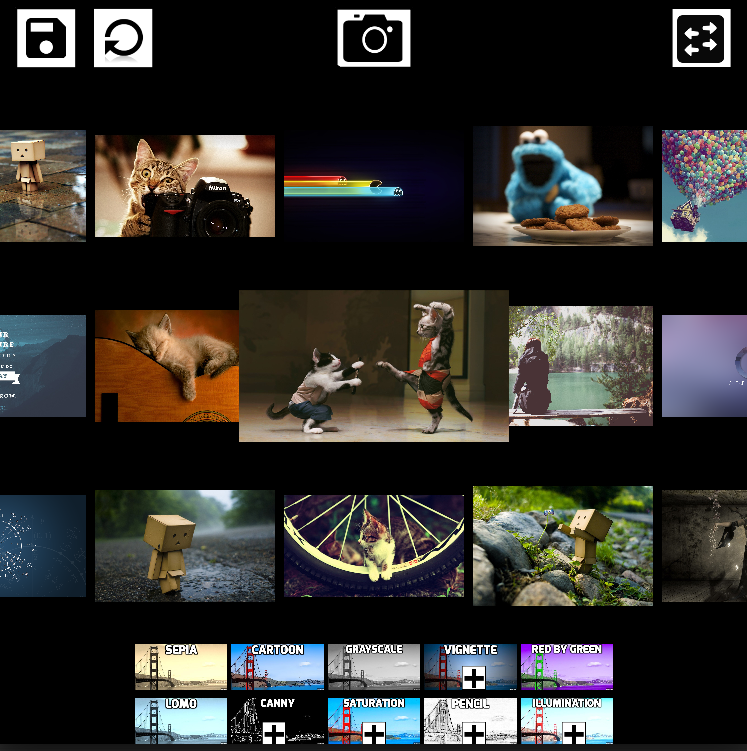
\includegraphics[width=230pt]{images/slideflow.png}}
\caption{Slideflow}
\label{img:complete}
\end{figure}

\section{Resultado Final}

O resultado final obtido foi o pretendido, sendo que é possível aplicar filtro sobre as imagens, utilizar a webcam aplicando filtros sobre a mesma, guardar a imagem seleccionada.\\

Um exemplo da imagem da webcam com o filtro aplicado em que a frente da webcam tem uma mão a segurar num telemóvel, mas com o filtro de Pencil Sketch.

\begin{figure}[H]
\centerline{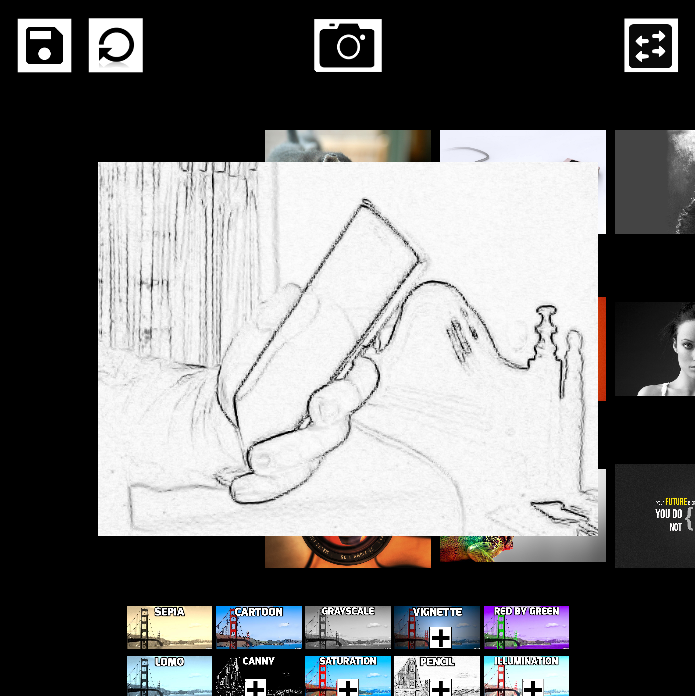
\includegraphics[width=230pt]{images/camera.png}}
\caption{Camera com Pencil Sketch}
\label{img:complete}
\end{figure}

Também se pode verificar que a função de zoom utilizado o scroll pode dar jeito para ver uma imagem com melhor resolução.

\begin{figure}[H]
\centerline{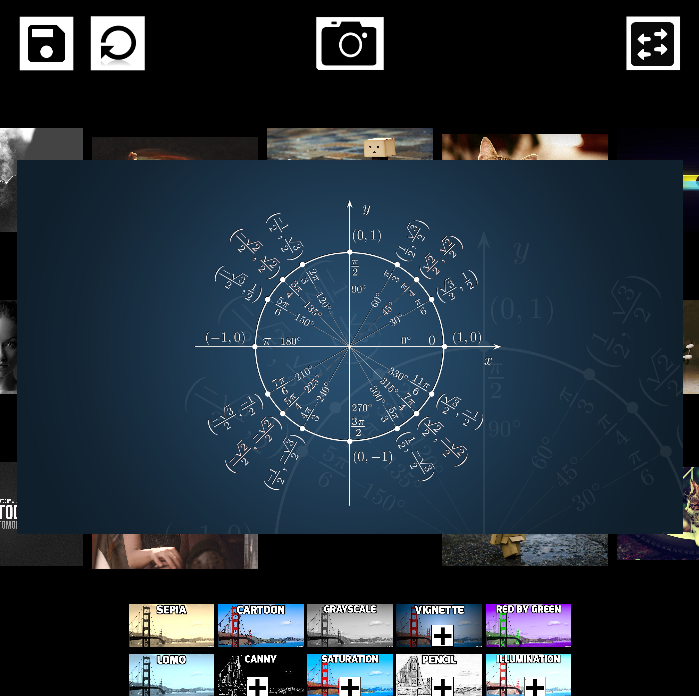
\includegraphics[width=230pt]{images/zoom.png}}
\caption{Zoom in}
\label{img:complete}
\end{figure}

Sendo este o resultado final obtido na aplicação.

\section{Compilação e Execução}

Código fonte disponível em:

{\tt \url{https://github.com/dbtds/slideshow3d-cvgl}}

Podendo ser obtido através do comando: {\tt git clone https://github.com/dbtds/slideshow3d-cvgl.git}

Este projecto foi desenvolvido unicamente em ambiente Linux, sendo assim, não foi criado qualquer ficheiro executável para ambiente Windows, apesar que também é possível faze-lo alterando apenas a forma de compilação.\\

Note-se que todas as próximas indicações foram apenas realizadas em ambiente Linux no Ubuntu 14.04 64 bits.\\

Software essencial para compilar e correr o programa:
\begin{enumerate}
\item build-essential
\item qt4-qmake
\item libglew-dev
\item freeglut3-dev
\item libboost-system-dev
\item libboost-filesystem-dev
\item opencv (pode-se ter que compilar esta biblioteca a partir do source)
\end{enumerate}

Para obter cada dependência basta executar:

{\tt sudo apt-get install dependency\_name}

Após a obtenção de todas estas dependências, basta executar o Makefile na pasta principal (root).

Executando em bash {\tt / \$ make}

Para executar o programa, basta ir a pasta gerada bin, e correr o executável com o nome chess.
Executando em bash {\tt /bin \$ ./slideshow3d example\_images/}

Já existe um executável pré-gerado apenas para 64 bits dentro da pasta bin com o nome chess\_bin64, executando da mesma forma:
Em bash {\tt /bin \$ ./slideshow3d\_bin64 example\_images/}


\bibliography{report} % use a field named url or \url{} for URLs
%\url{www.ua.pt}
% Note: the \bibliographystyle is set automatically

\end{document}
